\documentclass[conference,12pt]{IEEEtran}
\IEEEoverridecommandlockouts
% The preceding line is only needed to identify funding in the first footnote. If that is unneeded, please comment it out.
\usepackage{amsmath,amssymb,amsfonts}
\usepackage{algorithmic}
\usepackage{graphicx}
\usepackage{textcomp}
\usepackage{xcolor}
\usepackage{float}
\usepackage{listings}
\usepackage[backend=biber]{biblatex}

\addbibresource{references.bib}

\begin{document}

\title{Training a Neural Net to Recognize Tor Traffic}

\author{\IEEEauthorblockN{Cory Ness}
\IEEEauthorblockA{\textit{Department of Computer Science} \\
\textit{Kettering University}\\
Flint, Michigan, USA \\
ness2627@kettering.edu}
\and
\IEEEauthorblockN{Kyle David Prichard}
\IEEEauthorblockA{\textit{Department of Computer Science} \\
\textit{Kettering University}\\
Flint, Michigan, USA \\
pric8603@kettering.edu}
}

\maketitle

\begin{abstract}
This paper describes how successful it is to train a neural network to detect Tor traffic. It goes over the various network statistics that were found to be useful in determining if traffic is Tor-related, and how successful a fully trained neural network is in determining if traffic is Tor-related. It was found that using an autoencoder neural network for reconstructing traffic statistics provided accurate classification of Tor and Non-Tor traffic, achieving over $\%98$ accuracy in the test cases used. 
\end{abstract}

\begin{IEEEkeywords}
Tor, Tor Detection, Neural Network, Wireshark, TShark, Autoencoder, Reconstruction
\end{IEEEkeywords}

\section{Introduction}
Tor is commonly used to anonymize users for both legitimate and illegitimate purposes. In addition, Tor is used in malware, having the infected PC communicate with a control server over the Tor network. Because of this, it is useful to determine if Tor activity is happening on a local network to further scrutinize and determine if the activity is legal or illegal. This causes issues, however, because Tor traffic is not very different from regular traffic. There is no guaranteed IP that Tor traffic has to access, nor any guaranteed port, nor a guaranteed time or anything to definitively prove out that traffic is related to Tor activity. However, while there is nothing to definitively prove all this out, Tor traffic is noticeable in a few, more soft ways that can be defined and used in different detection methods to gain confidence that network is either Tor related or not.

\section{How Tor works}
Tor anonymizes users by routing traffic through multiple randomly selected Tor nodes before its' destination.  Each node only knows which relay it received data from and which to send it to, shown in figure \ref{fig:how-tor-works}.  According to Tor's own website, it "is similar to using a twisty, hard-to-follow route in order to throw off somebody who is tailing you - and then periodically erasing your footprints." \parencite{cite:Tor-Overview}

\begin{figure}[H]
    \centering
    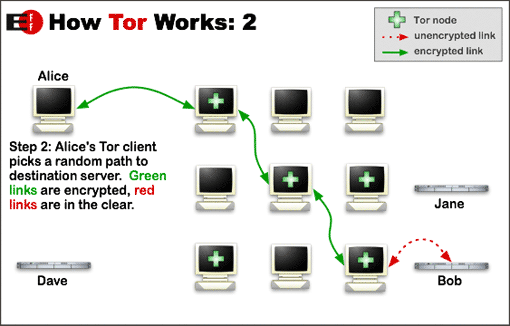
\includegraphics[scale=0.45]{Explanations/How-Tor-Works.png}
    \caption{An example of how Tor routes traffic through random nodes \parencite{cite:Tor-Overview}}
    \label{fig:how-tor-works}
\end{figure}

This routing through various nodes makes it nearly impossible for either a website to know who it is talking to or anyone sniffing the network connection to know what website you're browsing. This secures a large amount of anonymity for the user, and allows them to access materials that would otherwise be blocked.

However, since Tor is otherwise using completely legal and non-exploitative ways of securing these connections, it becomes difficult to know what traffic is typical traffic such as video streaming and what traffic is Tor traffic which could be illegal. 

\section{What is a Neural Network}
Neural networks are typically used to train a computer to do some task, and consist of a series of simple processing nodes connected to each other.  A nodes' connections will each have a weight assigned, and when data is received the node decides whether to pass the data on to the next node based on the data and the associated weight compared to a threshold value.  During training the weights and thresholds are set randomly, and they are adjusted until the network outputs desired values \parencite{cite:Explained-Neural-Networks}.

\section{Methods of Detecting Tor traffic}

It should be noted that Tor provides a DNS service which can be used to tell if traffic is coming from a Tor exit node \parencite{cite:Tor-Site}.  If the goal of detecting Tor traffic is just to block it this is a useful resource, though there are ways around even this through the use of unlisted nodes. Actually detecting Tor traffic is currently achieved through various means. The first of these is the method we chose, using a neural network to monitor statistics of network traffic and classify it as Tor or non-Tor related. There are other methods, such as using a neural network to monitor the encrypted data and check for malicious website fingerprints, flagging a packet in real-time if it contains a malicious fingerprint \parencite{cite:Adaptive-Onsite-Website-Fingerprinting}, and to monitor the raw traffic and run it through the neural network \parencite{cite:Machine-Learning-Tor-Detection}. These other methods are better for real-time classification of the network traffic, since they perform analysis on a smaller time frame, and possibly on individual packets, but they provide successful rates of around $\%90$, which provides a fair amount of uncertainty in classifying some traffic as benign or malignant.

\section{How we detected Tor traffic}
We detected Tor traffic by training an autoencoder neural network on various network statistics that were calculated after a period of time of network traffic was captured. We then checked to see if at any given second there was Tor network traffic. The neural network was trained on a benign data set that consisted of transferring a file over SFTP, while it compared against malicious data that consisted of a file transfer over SFTP using Tor. These two use cases are very similar, with the only exception being that Tor is used in the malicious data set, so it would prove useful to determine if the neural network was able to detect the anomalous Tor activity.

The networks statistics that were used to determine if network activity was Tor related or not were the following in 1-second intervals:
\begin{enumerate}
    \item Total Packet Length
    \item Total Number of Packets
    \item Inter Arrival Time
    \item Window Size
    \item Window Size Scalefactor
    \item Window Size Value
    \item Syn Flag
    \item Ack Flag
    \item Res Flag
    \item Push Flag
    \item Source Port Entropy
    \item Destination Port Entropy
\end{enumerate}

In order to gain the statistics, a pcap file was provided and ran through a python script that used Tshark to scan through the file, filter it to just the traffic concerning one local IP, and performed analysis to get the relevant properties of each packet. This script would output a csv file with all the properties of every packet, which was then fed into a merging script. The merging script batched all the rows by some common property, in this case it was batched so every point was 1 second and contained the sum of all the properties beforehand. In addition, it would perform more complex analysis, such as entropy calculation of the source and destination ports using the following python code:

\begin{lstlisting}[language=Python, breaklines=true]
for index, row in df.iterrows():
    packet_count += 1 # Increment packet count for new packet
    src_port = row["Source_Port"]
    if not src_port in src_port_calculation:
        src_port_calculation[src_port] = 0
    src_port_calculation[src_port] += 1
    dst_port = row["Source_Port"]
    if not dst_port in dst_port_calculation:
        dst_port_calculation[dst_port] = 0
    dst_port_calculation[dst_port] += 1
    if row["Timestamp"] != last_timestamp or (index + 1) == total:
        last_timestamp = row["Timestamp"]
        src_port_entropy_tmp = 0
        dst_port_entropy_tmp = 0
        for key, p in src_port_calculation.items():
            src_port_entropy_tmp += -(p / packet_count) * math.log2(p / packet_count)
        for key, p in dst_port_calculation.items():
            dst_port_entropy_tmp += -(p / packet_count) * math.log2(p / packet_count)
        packet_count = 0
        src_port_calculation = {}
        dst_port_calculation = {}
        src_port_entropy.append(src_port_entropy_tmp)
        dst_port_entropy.append(dst_port_entropy_tmp)
\end{lstlisting}

Based on previous work in \parencite{cite:Tree-Based-Models}, we expected \texttt{Window Size} to be the most significant contributor to the neural network, with lesser importance in \texttt{Source Port Entropy} and \texttt{Destination Port Entropy}. This is because the window size is relatively constant for traffic routing through Tor, matching up to multiples of some constant. This is much more different than normal traffic, where the window size is adjusted to best fit whatever is being sent between devices, always changing and seemingly random from an outside observer. Along with that, we'd expect port entropy to be a contributing factor because the ports that Tor uses should change at a wider level than normal traffic. Tor has taken steps to reduce its footprint in this regard, which is where \parencite{cite:Tree-Based-Models} makes note that port entropy is no longer the most sound method of classifying Tor and non-Tor traffic. The other statistics that were added may or may not help the model, but since this is an autoencoder neural network, it cannot hurt the model except in time taken to optimize, so little research was done on whether to include or exclude them in the training.

The manner in which we trained the neural network was through reconstruction. The neural network will try to reconstruct data based on statistics of some traffic, and if it's close to the actual data, it will be classified as benign data. However, if the reconstructed data is far from the actual data, the data will be considered malignant, or in other words, is Tor traffic. An example of reconstruction is shown in figure \ref{fig:reconstruction}. The neural network was trained for 60 generations on the benign traffic statistics, attempting to most closely reconstruct the traffic so that traffic that does not match the reconstruction is declared maligned and classified as Tor-related.

\begin{figure}[H]
    \centering
    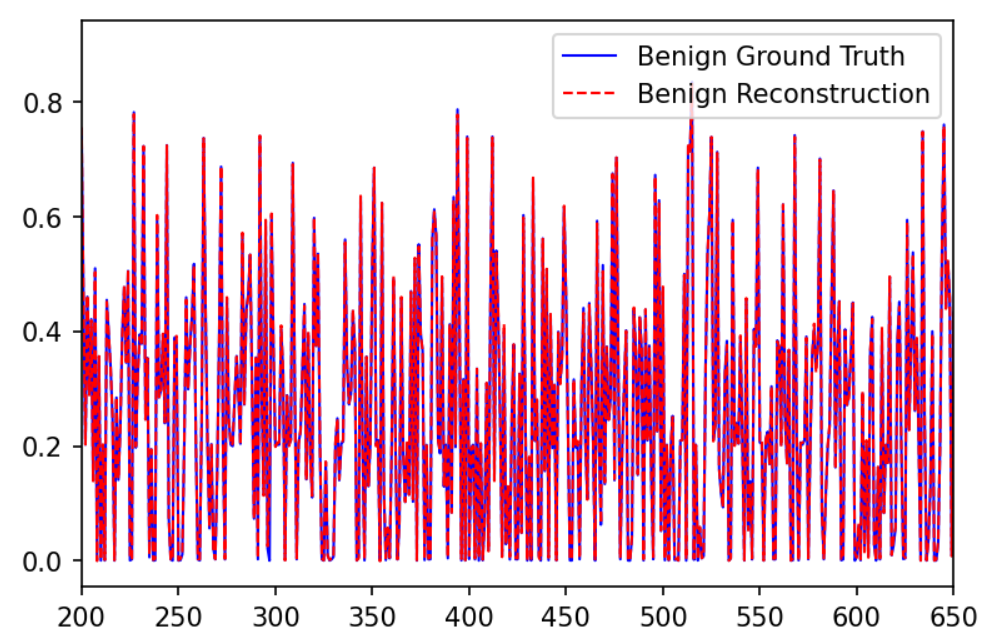
\includegraphics[scale=0.4]{Project-Results/Benign-Reconstruction.png}
    \caption{An example of the neural network reconstructing data based on a benign data set.}
    \label{fig:reconstruction}
\end{figure}

\section{Analysis of Neural Net Training}
With the method discussed above, we had significant success in determining if traffic was Tor related or not. This is shown in both figures \ref{fig:confusion-matrix}, \ref{fig:reconstruction-error}, and \ref{fig:mse-loss}. Figure \ref{fig:confusion-matrix} details exactly what data points were successfully determined to be benign/maligned, and what points were incorrectly determined benign/maligned. In this case, 1173 of 1176 points were correctly identified benign, and 1229 of 1234 points were correctly identified malign. Using the formula $P_{Correct}= \frac{N_{Correct}} {N_{Total}}$, we get a true positive rate of $\frac{1173}{1176} = \%99.74$ and a true negative rate of $\frac{1229}{1254} = \%98.00$. Overall, this method is $\frac{2402}{2430} = \%98.84$ correct.

\begin{figure}[H]
    \centering
    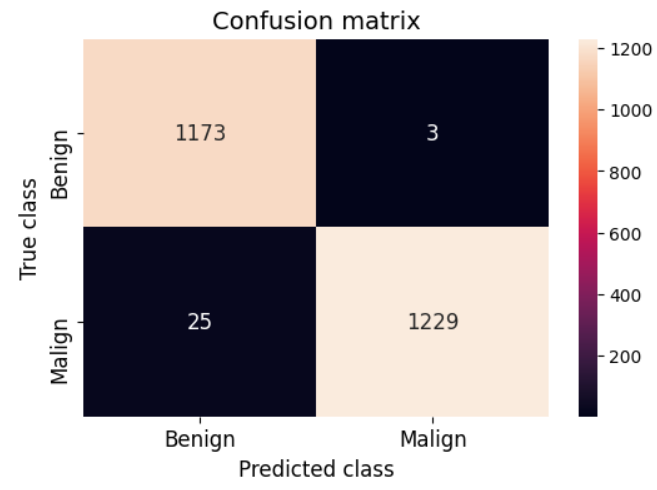
\includegraphics[scale=0.63]{Project-Results/Confusion-Matrix.png}
    \caption{Confusion Matrix showing the accuracy of the neural network that was trained with provided statistics.}
    \label{fig:confusion-matrix}
\end{figure}

Another way to look at the results of the training is by looking at figure \ref{fig:reconstruction-error}, where the data points are characterized by their mean-square-error loss. Two types of data points are plotted, with orange being the maligned data and blue being the benign data. If a point is above the dashed line, it is characterized as maligned, and if it's below it is characterized as benign. This figure shows how the vast majority of benign dots are below the dashed line and orange dots are above the dashed line, but it also shows how there are some data points that are incorrectly above or below the dashed line. These misplaced dots are the false positive and false negative data points, and while there are a good few, they are by far in the minority when compared to the massive number of points that are correctly identified.

\begin{figure}[H]
    \centering
    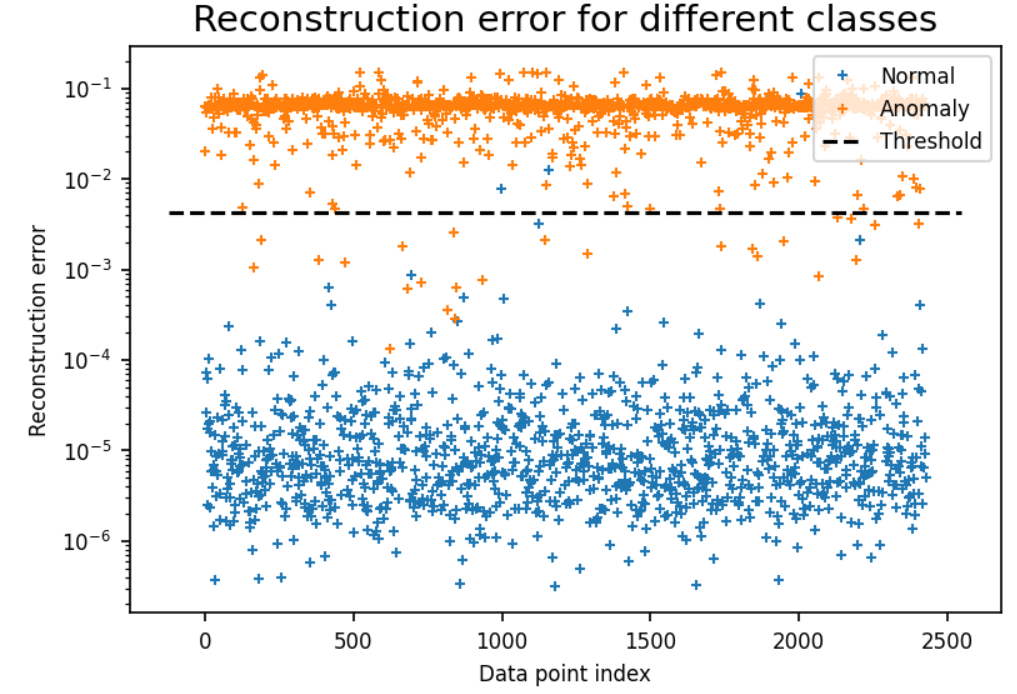
\includegraphics[scale=0.4]{Project-Results/Reconstruction-Error.png}
    \caption{Reconstruction error showing accuracy of the neural network that was trained with provided statistics}
    \label{fig:reconstruction-error}
\end{figure}

Similarly to figure \ref{fig:reconstruction-error}, figure \ref{fig:mse-loss} shows the reconstruction error, but in this case it's bar-plotted with the x-axis indicating the loss. The further to the left of the plot, the more likely it is to be benign data. In this case, the maligned data is so far to the right it's nearly impossible to look at it in clarity, and shows just how poor the maligned data fits with the reconstructed data in most cases.

\begin{figure}[H]
    \centering
    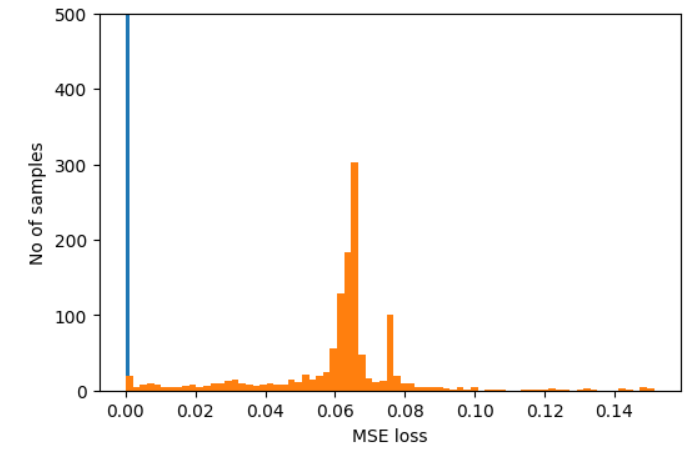
\includegraphics[scale=0.6]{Project-Results/MSE-Loss.png}
    \caption{Graph showing the Mean Square Error loss of the benign data set (blue) and maligned data set (orange). Further to the left indicates closer reconstruction and therefore more likely to be benign.}
    \label{fig:mse-loss}
\end{figure}


\section{Conclusion}
The results of the project were very promising, we were able to achieve results similar to \parencite{cite:Tree-Based-Models}, getting in the high ninety percentage for accuracy. As well, there were few false positives and false negatives, suggesting that this method could be used in some form of automation such as logging without worrying too much about clutter and missed traffic. Finally, since this method makes use of MSE, it is possible to tighten the parameters to allow fewer false-positives or false-negatives at the cost of the other, so that it can be tweaked to best accommodate a specific application.

\printbibliography

\end{document}
